\documentclass[twocolumn]{article}
\usepackage{amsmath}
\usepackage{xcolor}
\usepackage{graphicx}
\usepackage{caption}
\usepackage{fancyhdr}
\usepackage{geometry}
\usepackage{enumitem}
\usepackage{array}
\usepackage{hyperref}
\geometry{margin=0.7in}
\pagestyle{empty}

\begin{document}

\begin{figure}[t]
    
\includegraphics[width=\linewidth]{img3.png} % Uploaded image
        \textbf{Name: K.Saisusmitha} \\
    \textbf{Batch: 2} \\
    \textbf{ID: cometfwc018} \\
    \textbf{Date: 9th July 2025}
\end{figure}

\begin{center}
    {\LARGE \textbf{\textcolor{blue}{GATE Question Paper 2010, PH Question Number 41}}}
\end{center}

\vspace{1em}
\begin{figure}[h]
    \centering
    \includegraphics[width=0.8\linewidth]{ph2010 41.png}
        \caption*{\textbf{Figure: Logic Gate Circuit}}
\end{figure}

\section*{\textcolor{blue}{Question Analysis}}
\textbf{Given:} Four different logic circuits labeled (A) to (D) are presented.  
\textbf{Task:} Identify which one of the circuits gives a different output $Q$ compared to the others.

\section*{Solution}

Let’s evaluate the logic expression for each option:

\begin{enumerate}[label=\textbf{Option (\Alph*):}]
    \item \textbf{(A)}  
    \[
    \text{Q}_A = \overline{(A + B)} \cdot \overline{A}
    \]

    \item \textbf{(B)}  
    \[
    \text{Q}_B = \overline{A} \cdot \overline{B} = \overline{(A + B)} \quad \text{(By De Morgan's Law)}
    \]

    \item \textbf{(C)}  
    Two expressions:
    \begin{align*}
    X &= \overline{A} \cdot B \\
    Y &= \overline{B} \cdot A \\
    \text{Q}_C &= X + Y = A \oplus B
    \end{align*}

    \item \textbf{(D)}  
    \[
    \text{Q}_D = \overline{A} + B
    \]
\end{enumerate}

\textbf{Now compare:}  
- (A), (B) simplify to: $\text{Q}_A = \overline{(A + B)} \cdot \overline{A}$ — not equal to others directly.  
- (B) gives $\overline{(A + B)}$  
- (C) is clearly $A \oplus B$  
- (D) is $\overline{A} + B$

\textbf{Conclusion:} Circuit (C) gives XOR output, while others are variations of NOR or combinations thereof.  
Hence, **(C)** is the different one.

\section*{\textcolor{blue}{Correct Option: (C)}}

\section*{\textcolor{blue}{Truth Table}}

\begin{table}[h]
\centering
\renewcommand{\arraystretch}{1.3}
\begin{tabular}{|c|c|c|c|c|c|}
\hline
A & B & Q\textsubscript{A} & Q\textsubscript{B} & Q\textsubscript{C} & Q\textsubscript{D} \\
\hline
0 & 0 & 1 & 1 & 0 & 1 \\
0 & 1 & 0 & 0 & 1 & 1 \\
1 & 0 & 0 & 0 & 1 & 0 \\
1 & 1 & 0 & 0 & 0 & 1 \\
\hline
\end{tabular}
\caption*{\textbf{Table: Comparison of Outputs for Each Circuit}}
\end{table}

\section*{\textcolor{blue}{Hardware Implementation Idea}}

You can simulate and verify each option (A–D) using:
\begin{itemize}
    \item Raspberry Pi Pico or Arduino Uno
    \item Push buttons for A and B
    \item LEDs for output $Q$
\end{itemize}

Implement each logic function in code or hardware gates and compare outputs for all four input combinations of A and B.

\section*{\textcolor{blue}{Conclusion}}
\begin{figure}[h]
    \centering
    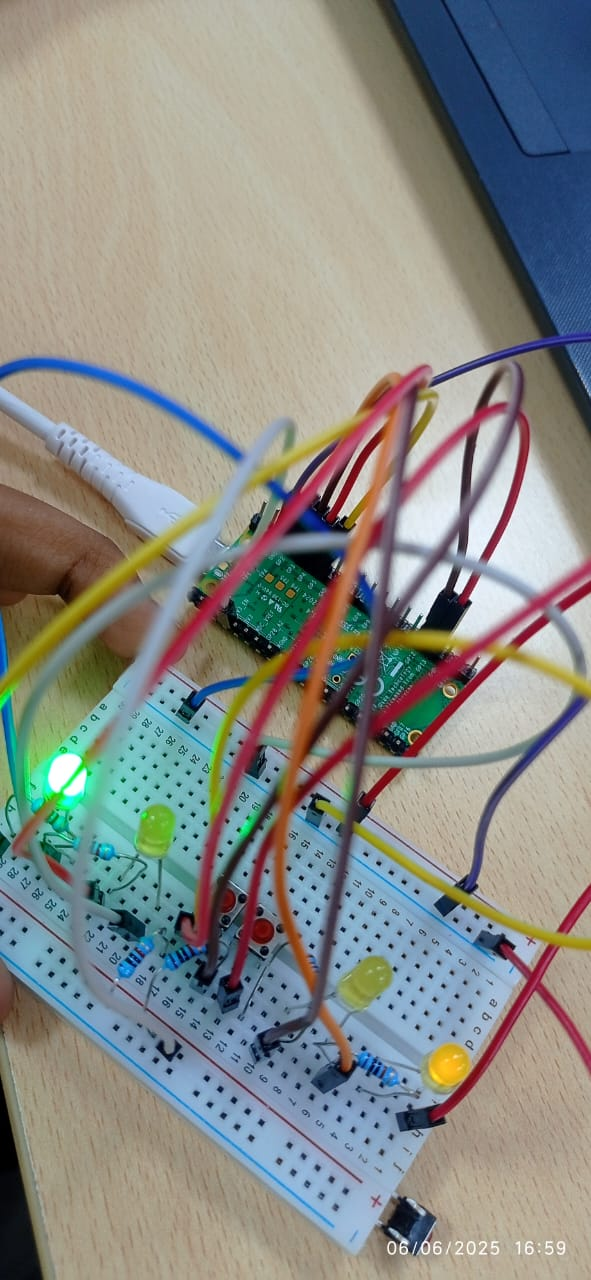
\includegraphics[width=0.9\linewidth]{avr_gcc.jpg}
        \caption*{\textbf{Figure: Representative Logic Circuit Setup}}
\end{figure}

From analysis and truth table comparison, we find:
\[
\boxed{\text{Option (C) is the odd one out as it implements XOR logic}}
\]

\section*{\textcolor{blue}{Source Code Link}}
The complete hardware simulation and code implementation for this experiment is available at the following GitHub repository:

\textbf{GitHub Repo:} \href{https://github.com/aisusmitha/FWC.git}{github.com/aisusmitha/FWC.git}
\end{document}
